\documentclass[12pt,fleqn,a4paper,nodisplayskipstretch]{article}
\usepackage[utf8]{inputenc}
\usepackage[a4paper, left=30mm, right=20mm, top=30mm, bottom=20mm]{geometry}
\usepackage{ragged2e}
\usepackage{mathptmx}

\usepackage{fancyhdr}
\usepackage{quoting}
\usepackage{nomencl}
\usepackage[brazil]{babel}



\usepackage{bezier,amstext,amsthm,makeidx,indentfirst,ifthen,cite,minitoc}

\usepackage[]{setspace}

\usepackage[alf,abnt-repeated-title-omit=yes,abnt-emphasize=bf,abnt-etal-list=0]{abntex2cite}


\citebrackets()
\makenomenclature

\renewcommand{\footnoterule}{
\kern -3pt
\hrule width 5cm
\kern 2pt
}

\AtBeginDocument{
    %Centralização do título sumário
    \renewcommand\contentsname{\centering \normalsize \uppercase{Sumário}}
    %Renomeação do título das siglas
    \renewcommand{\nomname}{\centering \normalsize \uppercase{Siglas}} 
    %Remoção do título referências
    \renewcommand{\refname}{} 
    %Renomeação do título da lista de figuras
    \renewcommand{\listfigurename}{\centering \normalsize \uppercase{Lista de figuras}}
    %Renomeação do título da lista de tabela
    \renewcommand{\listtablename}{\centering \normalsize \uppercase{Lista de tabela}}
}

\pagestyle{fancy}
\fancyhf{}
\fancyheadoffset{0cm}
\renewcommand{\headrulewidth}{0pt} 
\renewcommand{\footrulewidth}{0pt}
\fancyhead[R]{\thepage}
\fancypagestyle{plain}{
  \fancyhf{}
  \fancyhead[R]{\thepage}
}


\begin{document}
\pagestyle{empty}
\begin{center}
\bf{Universidade Estadual Paulista ``Júlio de Mesquita Filho''}
  
  \bf{FCT — Faculdade de Ciências e Tecnologia}
  
  \bf{DMC — Departamento de Matemática e Computação}
  
  \bf{Bacharelado em Ciência da Computação}
  
  \vspace*{\fill}
  \vspace{42pt}
  \Large{	\textmd{Trabalho de Conclusão de Curso}}
    
  \large{Anteprojeto de pesquisa}
  
  \vspace{42pt}
  \Large{Aplicação de métodos de Inpainting em imagens digitais}
  
  \vspace{42pt}
  \normalsize{\bf{Gustavo Becelli do Nacimento}
  
  \vspace{12pt}
  Orientador: \textmd{Prof.\ Dr.\ Almir Olivette Artero}}
  
  \vspace*{\fill}
  \vspace{12pt}
  Presidente Prudente, 22 de janeiro de 2023
\end{center}
\pagebreak

\pagenumbering{arabic}
\tableofcontents{}
\pagebreak

% \section*{Resumo}
O inpainting de imagens é a técnica de modificar imagens com aplicação majoritariamente concentrada em restauração de imagens corrompidas por ruídos, borrões, arranhões, objetos indesejados, textos sobrepostos (e.g. legendas e marcas-d’-água), defeitos da lente de captura, entre diversas outras falhas em imagens digitais. 

Os métodos estabelecidas para aplicar o inpainting podem ser divididos em duas categorias: (1) métodos sequenciais clássicos, e (2) métodos baseados em aprendizado, que utilizam redes neurais convolucionais (CNNs) e/ou Redes Generativas Adversárias (GANs). A primeira categoria ordinariamente possui métodos mais leves, que recorrem às equações diferenciais parciais (PDEs), enquanto as duas últimas, para obterem melhores resultados, utilizam maior processamento computacional e necessitam de treinamento prévio para ajustar seus parâmetros.

Este trabalho desenvolverá este tema e apresentará uma revisão teórica dos métodos de inpainting, aprentado algumas das técnicas e conceitos principais utilizados. Como resultado, foi possível compreender que os métodos clássicos são, em geral, mais rápidos e eficientes, mas apresentam resultados menos realistas e borramentos. Por outro lado, os métodos baseados em aprendizado são mais lentos e computacionalmente mais custosos, mas apresentam resultados mais plausíveis. Apesar disto, em geral, todos costumam considerar as regiões vizinhas ou semelhantes para preencher a região alvo.

Palavras-chave: Inpainting, processamento de imagens, preenchimento de regiões, aprendizado de máquina.
\pagebreak
\section*{Abstract}
Image inpainting is a technique for modifying images with application mainly focused on restoring images corrupted by noise, blurs, scratches, unwanted objects, superimposed texts (e.g. subtitles and watermarks), capture lens defects, among others. several other flaws in digital images.

The established methods for applying inpainting can be divided into two categories: (1) classical sequential methods, and (2) learning-based methods, which use convolutional neural networks (CNNs) and/or Generative Adversarial Networks (GANs). The first category ordinarily has lighter methods, which resort to partial differential equations (PDEs), while the last two, in order to obtain better results, use more computational processing and require prior training to adjust their parameters.

This work will develop this theme and present a theoretical review of inpainting methods, presenting some of the techniques and main concepts used. As a result, it was possible to understand that the classical methods are, in general, faster and more efficient, but present less realistic results and blurring. On the other hand, learning-based methods are slower and computationally more expensive, but present more plausible results. Despite this, in general, everyone usually considers neighboring or similar regions to fill the target region.

Keywords: Inpainting, image processing, region filling, machine learning.
% \pagebreak

% Apresentar uma panorâmica da área a ser estudada, descrevendo o histórico da área, o cenário atual, os problemas existentes, o objetivo deste trabalho e, no final, a estrutura deste documento, descrevendo brevemente os demais capítulos desta revisão.

\section{Introdução} \label{introduction}
O Inpainting  de Imagens é o processo de preencher regiões faltantes ou danificadas de uma imagem com o intuito de restaurá-la ou melhorar sua aparência. Este é um problema amplamente estudado em visão computacional e possui uma vasta gama de oportunidades de aplicações, incluindo o restauro de obras artísticas e fotografias danificadas, a remoção de objetos de imagens e síntese de texturas~\cite{criminisi2004region}.

Esta área de pesquisa tem sido estudada há várias décadas. Os primeiros trabalhos sobre o tema surgiram na década de 1950, mas foi somente a partir dos anos 1990 que o inpainting começou a ser utilizado de maneira mais ampla.

\cite{Elharrouss2019} apresenta uma revisão sobre o inpainting de imagens, descrevendo os principais métodos e aplicações. Neste campo, existem várias técnicas para o inpainting de imagens, cada tal com suas próprias vantagens e desvantagens. Uma abordagem popular é apresentada em \cite{Bertalmio2000}, a qual introduz uma técnica de inpainting baseada no conceito de complementar uma região de uma imagem existente. Neste trabalho é utilizado equações diferenciais parciais para propagar informações das bordas da região danificada para o centro da região, permitindo que o algoritmo estime como os pixels devem ser restaurados.

Uma das contribuições mais significativas para o campo de inpainting de imagem é o desenvolvimento do ``Método de Marcha Rápida'' ~\cite{Telea2004}, um algoritmo eficiente que usa equações diferenciais parciais para propagar informações de pixels conhecidos para os pixels desconhecidos na região de inpainting. Este algoritmo tem sido amplamente utilizado em várias aplicações e foi implementado em muitas bibliotecas de software, incluindo a biblioteca de código aberto de visão computacional OpenCV \cite{OpenCV}. Este método tem demonstrado produzir resultados de alta qualidade para uma ampla variedade de tipos de imagem e cenários, e se tornou uma das referências para avaliar o desempenho de outros algoritmos de inpainting.

Nos últimos anos, houve um aumento de interesse em utilizar métodos baseados em aprendizado de máquina, como redes adversárias gerativas (GANs) e redes neurais convolucionais (CNNs) \cite{pathakCVPR16context}, para resolver o problema de inpainting. Esses métodos têm o potencial de aprender padrões e estruturas complexas a partir de grandes conjuntos de dados, o que pode ser usado para gerar resultados de inpainting de alta qualidade. No entanto, esses métodos podem ser computacionalmente caros e podem exigir uma abundância de dados de treinamento para obter bons resultados.

Hoje, o inpainting é utilizado em uma variedade de aplicações. Dentre elas, está incluída o restauro de obras de arte danificadas, a remoção de objetos de imagens (como nuvens em imagens de sensoriamento remoto) e até mesmo a
remoção de imperfeições de fotografias. Além disso, pode-se utilizar os mesmos conceitos de restauração para modificar as perspectivas de imagens, como é apresentado em \cite{huang2014image}.

O principal problema encontrado neste campo de pesquisa são a escolha do método de inpainting mais adequado para cada tipo de imagem e cenário. Este fator se deve às desvantagens que os métodos existentes proporcionam \cite{Salem2021}. Em geral, os maiores desafios são:
\begin{itemize} 
  \item \textbf{Preservação da consistência e estrutura da imagem de entrada:} muitos modelos geradores podem gerar imagens visualmente agradáveis, mas que não correspondem perfeitamente com a vizinhança ou à textura da imagem original.
  \item \textbf{Preservação de pequenos detalhes:} este problema é particularmente desafiador para imagens com texturas complexas, como imagens de paisagens naturais, ou a área que está sendo restaurada é muito grande.
  \item \textbf{Reconstruir objetos sobrepostos:} quando um objeto é parcial ou completamente sobreposto, como um objeto que está coberto por uma nuvem, o modelo gerador pode não ser capaz de reconstruir o objeto original.
  \item \textbf{Preenchimento de grandes regiões:} a geração de imagens de alta qualidade quando há uma grande região a ser reconstruída ainda é um problema desafiador.
  \item \textbf{Desempenho computacional:} a maioria dos métodos de inpainting de imagens que geram imagens de alta qualidade são computacionalmente caros, dificultando sua aplicação em tempo real.
\end{itemize}


\subsection{Objetivos}

\subsubsection{Objetivo principal}
O objetivo principal deste Trabalho de Conclusão de Curso é investigar e implementar algumas das diferentes técnicas de Inpainting para a restauração de imagens digitais com defeitos ou objetos indesejados. Para alcançar esse objetivo, serão estudadas técnicas clássicas baseadas em informações de vizinhança e amostras, bem como técnicas mais recentes baseadas em aprendizado de máquina. Além disso, serão aplicadas as técnicas estudadas em diversos tipos de imagens para avaliar sua eficácia e comparar os resultados obtidos.

\subsubsection{Objetivos secundários}
\begin{itemize}
  \item Estudar alguns dos principais métodos de inpainting, com o intuito de entender como cada um deles funciona e quais são suas vantagens e desvantagens.
  \item Aplicar as técnicas de inpainting estudadas em diversos tipos de imagens, incluindo imagens coloridas, imagens de alta resolução e imagens com diferentes tipos de defeitos, como buracos, riscos, manchas, etc.
  \item Aperfeiçoar os conhecimentos em processamento de imagens e aprendizado de máquina do aluno, bem como a capacidade de aplicar esses conhecimentos em problemas reais.
  \item Estudar a possibilidade de melhorias na eficácia (qualidade das imagens geradas) e na eficiência (tempo de processamento, uso de memória) dos métodos de inpainting estudados.
\end{itemize}

Os três objetivos secundários representam o âmbito deste trabalho dentro do objetivo principal. O último, por sua vez, representa o interesse do aluno em aprofundar seus conhecimentos em otimização computacional de algoritmos e a possibilidade de contribuir com a comunidade científica.

\subsection{Organização do Trabalho}
Inicialmente apresenta-se uma fundamentação teórica sobre o processo de inpainting, incluindo uma breve introdução sobre o escopo de inpainting, as principais categorias da área e posteriormente uma revisão de alguns dos principais métodos utilizados.
Em seguida, há uma seção destinada a mencionar algumas possíveis técnicas de otimização computacionais que podem ser aplicadas caso haja a possibilidade de serem implementadas.

Por fim, é apresentado um 

\section{Fundamentação teórica}

A gama de aplicações processo de inpainting em imagens digitais é ampla, uma vez que não se limita a um único domínio de aplicação. Em adição ao uso na fotografia e design gráfico, a técnica pode ser aplicada em diversas áreas, tais como a medicina, engenharia, arquitetura, entre outras, as quais podem se beneficiar da correção de imagens com defeitos, lacunas ou que necessitem manipular informações de forma não intrusiva.

Além disso, o conceito de inpainting, inicialmente apresentado em (\ref{introduction}), não agrega apenas as ideias de restauração de imagens ou remoção de objetos, mas também a construção e reconstrução de imagens \cite{you2019pirec}, a preservação da privacidade (por exemplo, borramento de rostos e placas de veículos automotivos) em imagens públicas \cite{google2022magritte}, ao preenchimento de lacunas em imagens de satélites \cite{Maalouf2009bandelet}, entre outros possíveis usos, aos quais alguns serão mais explorados no prosseguir desta revisão. Por fim, o tópico (\ref{related}) apresenta os trabalhos relacionados ao tema. 

Neste trabalho, o escopo de inpainting de imagens pode ser compreendido como uma técnica utilizada para preencher regiões vacantes/danificadas ou remover objetos. O objetivo do inpainting é reconstruir as regiões afetadas de forma que o resultado seja o mais visualmente plausível possível, ou seja, que a imagem resultante seja natural à ótica humana e não apresente artefatos visuais, enquanto preserva a coerência e consistência da imagem original \cite{levin2003learning}.

Há diversas formas de se implementar o processo de inpainting, sendo que a escolha do método a ser utilizado depende do domínio de aplicação, das características da imagem, do tipo de máscara, entre outros fatores \cite{black2020evaluation}.
Apesar disto, é comum distinguir duas variedades de métodos amplamente utilizados: os métodos ``clássicos'', os quais geralmente utilizam informações da estrutura ou da imagem ou outras regiões para preencher lacunas, e os métodos baseados em aprendizado, os quais comumente utilizam grandes quantidades de dados para serem treinados, sendo que os métodos baseados em aprendizado são os mais recentes e apresentam geralmente resultados mais satisfatórios.

Em suma, o inpainting de imagem é uma técnica utilizada para preencher regiões faltantes ou corrompidas de uma imagem, como uma nuvem em uma imagem de sensoriamento remoto, ou danos causados pela degradação em fotografias digitalizadas, como na Figura \ref{fig:inpainting-couple}.

\begin{figure}[ht]
\centering
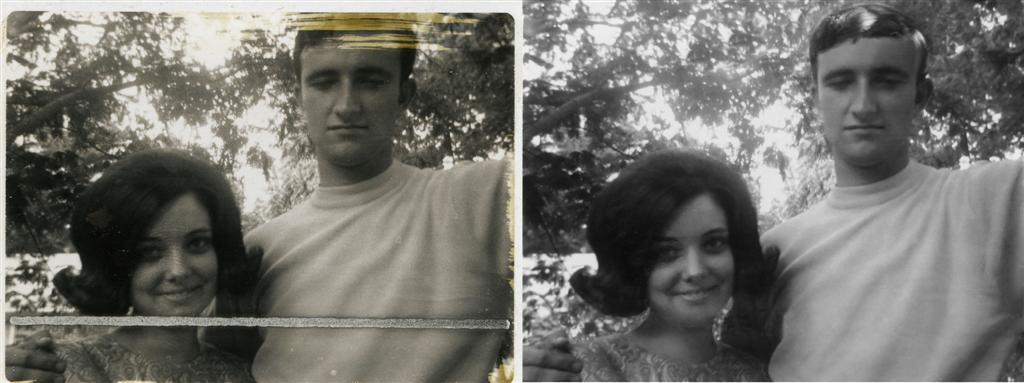
\includegraphics[width=1\textwidth]{inpainting-couple.jpg}
\caption{Exemplo do inpainting de imagens \cite{wiki:inpainting-couple}. A imagem da esquerda mostra uma imagem danificada. A imagem à direita mostra o resultado após o processo de inpainting.}
\label{fig:inpainting-couple}
\end{figure}


\subsection{Métodos clássicos} \label{patch}
Os métodos clássicos utilizam informações dos pixels e da região vizinha às regiões  vacantes ou danificadas para preenchê-las. Estes métodos são baseados no princípio de que regiões próximos e similares ao alvo são os mais adequados para preencher a região \cite{patchmatch2009, Bertalmio2001navier}.

É possível ainda, dentro desta estratégia, distinguir dois tipos de métodos: os métodos baseados em difusão, tais que propagam as informações próximas da região-alvo para preencher a lacuna, e os métodos baseados em patches e síntese de textura que utilizam amostras de regiões similares para preencher a lacuna.

\subsubsection{Métodos baseados em difusão} \label{diffusion}
Segundo \cite{black2020evaluation}, estes métodos transmitem os valores dos pixels adjacentes para as regiões a serem preenchidas e suas implementações são variadas. Métodos como \cite{Telea2004} utilizam uma o Método da Marcha Rápida, que consiste em propagar médias ponderadas das intensidades dos pixels adjacentes para a região-alvo, mantendo as altas e baixas frequências. Há outras implementações como \cite{Bertalmio2001navier}, que utilizam as equações de Navier-Stokes para a difusão de valores de pixels adjacentes e os isótopos (linhas com tons de cinza semelhantes) existentes. Estes métodos são simples e eficientes computacionalmente, porém, apresentam geralmente resultados com artefatos visuais, como bordas irregulares, texturas deformadas, etc, em especial, para imagens com texturas complexas.

\subsubsection{Métodos baseados em \emph{patches} (amostras)} \label{sample}
Estes métodos utilizam amostras de regiões conhecidas e similares a região-alvo para reconstruí-la. Assume-se que a região corrompida possui pixels semelhantes a alguma área próxima ou selecionada pelo usuário, então o método extrai esta amostra e a transfere para a região desejada, geralmente mantendo a coerência da imagem e a consistência visual. Essa estratégia é simples e eficiente computacionalmente, em especial para imagens com texturas e estruturas mais simples \cite{patchmatch2009}, simultaneamente, costumam apresentar resultados superiores aos de difusão. Em geral, não produzem resultados satisfatórios para lidar com imagens que contenham detalhes finos, imagens com bordas irregulares, imagens com objetos com texturas semelhantes, etc.

Dentro dos métodos baseados em patches, inclui-se os métodos baseados em síntese de texturas, os quais utilizam amostras de regiões conhecidas e similares a região-alvo para reconstruí-la. Contudo, estes métodos utilizam amostras de texturas para sintetizar novos pixels para a região-alvo. Estes métodos são baseados no princípio de que a textura de uma região é uma função de sua vizinhança, e assume que a área vizinha ao alvo possui texturas similares, o que viabiliza propagar as bordas e frequências para preenchimento. Utilizar esta estratégia pode produzir resultados satisfatórios para imagens com texturas mais complexas, embora ainda encontrem dificuldades para lidar com imagens com bordas ou padrões irregulares, imagens com objetos com texturas semelhantes, entre outras \cite{bertalmio2003texture}.

\subsubsection{Exemplos}

O trabalho de \cite{Bertalmio2000} apresenta uma técnica iterativa que não necessita de intervenção do usuário para selecionar a textura que deve ser utilizada para preencher a região danificada. O ótimo da técnica apresentada é preencher regiões próximas de fronteiras, onde há alta frequência. Apesar disso, o autor comenta que não se recomenda a utilização para grandes regiões de textura. O algoritmo utiliza a estrutura ao redor da região a ser restaurada para ir preenchendo seu contorno e reduzindo a área de referência, propagando a textura existente.

\cite{Telea2004} propõe uma técnica que propaga a suavidade e os detalhes da região vizinha conhecida. O autor estima a suavidade como a média ponderada das intensidades e cores dos pixels adjacentes. Para completar o ponto $p$ presente na borda $\partial \Omega$ da região $\Omega$ a ser preenchida, o algoritmo seleciona a vizinhança $\epsilon$ de $p$ e calcula o valor de $p$ como uma função desta vizinhança, ponderando os valores dos pixels adjacentes de forma a manter a suavidade e os detalhes da região vizinha conhecida. A Imagem \ref{fig:telea} apresenta este conceito visualmente. 

\begin{figure}[h]
\centering
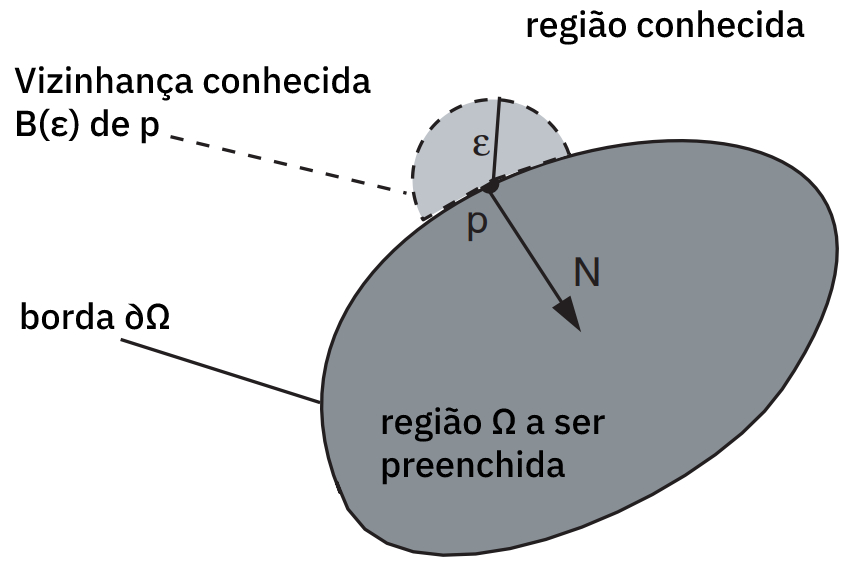
\includegraphics[width=0.7\textwidth]{inpainting-telea.jpg}
\caption{Adaptado de \cite{Telea2004}. A imagem retrata o princípio do inpainting para preencher um pixel.
} 
\label{fig:telea}
\end{figure}

\subsection{Métodos baseados em aprendizado} \label{learn-based}
Os métodos baseados em aprendizado, no que lhe concernem, utilizam técnicas de aprendizado de máquina, como redes neurais convolucionais (CNNs) e redes generativas adversárias (GANs) para preencher a região danificada. Estas técnicas "aprendem" a reconstruir a região danificada a partir de um conjunto de dados de imagens com e/ou sem máscara. Estes métodos são mais recentes e apresentam resultados mais satisfatórios, em especial para imagens com texturas complexas, imagens com bordas irregulares, imagens com objetos com texturas semelhantes, etc. Entretanto, eles geralmente são mais complexos e computacionalmente mais custosos, devido ao fato que de necessitarem de um grande conjunto de dados para serem treinados \cite{Goodfellow-et-al-2016}. Além disso, seu treinamento pode ser demorado, consoante o tamanho do conjunto de dados.

Nesta categoria existem diversos métodos existentes, utilizando diferentes técnicas de aprendizado de máquina e abordagem para o preenchimento. Apesar disto, os métodos podem ser divididos, mas não limitando-os, em dois grandes grupos: métodos baseados em CNNs e métodos baseados em GANs

\subsubsection{Métodos baseados em Redes Neurais Convolucionais} \label{cnn-based}
Estas espécies de métodos utilizam uma CNN para reconstruir as regiões faltantes. Eles se beneficiam da habilidade das CNNs de aprender as características de uma imagem e conseguem produzir bons resultados para imagens com texturas e estrutura complexas. A rede é treinada em um vasto conjunto de dados de imagens e aprende a reconhecer padrões e as características das imagens. Após o treinamento, a rede utiliza o conhecimento adquirido para gerar novos pixels para a região danificada, ainda preservando a região que a cerca.



\subsubsection{Métodos baseados em Redes Generativas Adversárias} \label{gan-based}
Estes métodos utilizam uma GAN para gerar novos pixels para preencher a região danificada. As GANs consistem em duas partes: uma rede geradora que gera novos pixels, e um discriminador que avalia a qualidade dos pixels obtidos~\cite{black2020evaluation}. Estes métodos podem gerar resultados mais realísticos do que os baseados em CNNs, ao custo de serem mais custosos computacionalmente e requererem um conjunto de dados maior para treinamento. Consequentemente, estes métodos costumam ser mais complexos e consumir mais tempo para treinamento \cite{pathakCVPR16context}.


\subsubsection{Exemplo}

O artigo de \cite{ren2015shepard} apresenta um método baseado em CNNs para inpainting em que a rede é treinada utilizando imagens tanto com quanto sem máscaras, o que possibilita que ela aprenda a reconstruir as áreas faltantes. Por se basear em \cite{shepard1968two} a máscara de convolução utilizada neste método leva em conta a distância espacial entre o pixel conhecido, que será utilizado como exemplo para a reconstrução, e o pixel a ser reconstruído, permitindo que a contribuição de cada pixel seja ponderada de forma apropriada. A figura \ref{fig:inpainting-convolution-mask.png} mostra um exemplo da máscara de convolução.

\begin{figure}[ht]
\centering
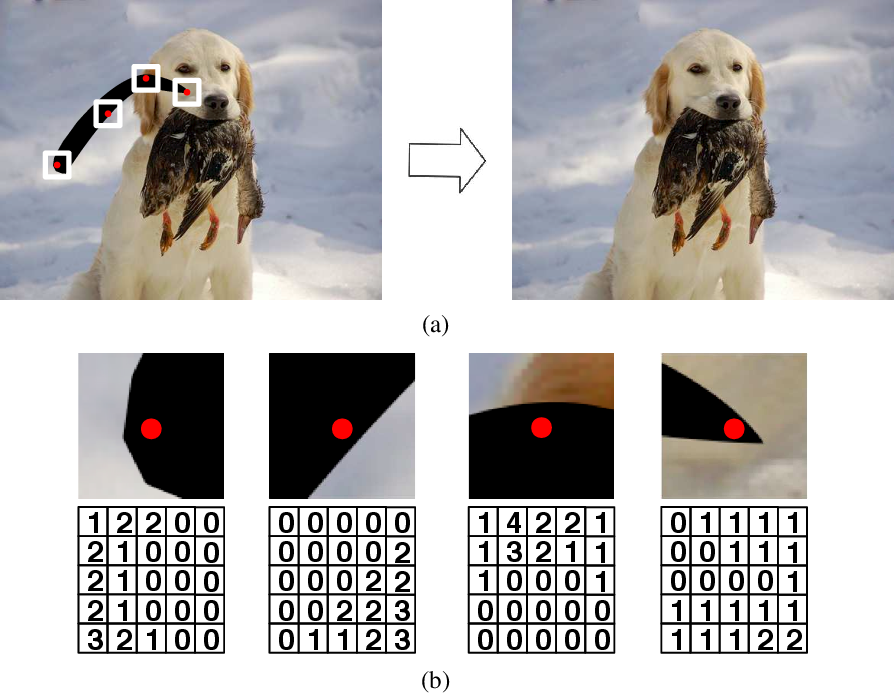
\includegraphics[width=1\textwidth]{inpainting-convolution-mask.png}
\caption{Adaptado de \cite{ren2015shepard}. (a) Aplicação do inpainting em uma imagem. (b) Máscara de convolução utilizada para reconstruir o ponto destacado na imagem.}
\label{fig:inpainting-convolution-mask.png}
\end{figure}



% TODO: Adicionar mais uma referência de GAN ou CNN para inpainting.


\section{Conceitos e técnicas} \label{concepts}

\subsection{Seleção da região} 
A escolha da região a ser preenchida é parte fundamental na qualidade do resultado do processo de inpainting, uma vez que ela afeta diretamente a qualidade dos resultados obtidos. A região selecionada deve abranger a região que se deseja preencher, mas não deve ser muito grande, pois isso pode levar a resultados com textura não realistas, consumir maior tempo de processamento ou até mesmo prejudicar a qualidade da imagem \cite{wang2020vcnet}.
Ademais, a região escolhida deve ser bem definida e conter uma delimitação clara, para que o algoritmo de preenchimento possa identificar com facilidade a região/estrutura a ser preenchida \cite{huang2014image}.

Alguns métodos realizam este processo de forma automática, sendo conhecidos por realizar um ``Inpainting cego'' (do inglês, \emph{Blind Inpainting}). O Trabalho de \cite{wang2020vcnet} apresenta um modelo discrinimativo para classificar os pixels da imagem e identificar as regiões inconsistentes com o conteúdo da imagem como, por exemplo, textos sobrepostos e rabiscos.

Por seguinte, é importante considerar a região que será preenchida, pois o processo de preenchimento pode afetar a coerência do resultado. Por exemplo, o preenchimento de uma região complexa ou que contém o conteúdo principal de uma imagem possui mais detalhes que precisam ser preservados ao comparar-se com o preenchimento de uma região de fundo.

A Figura \ref{fig:inpainting-region} mostra um exemplo da seleção de regiões para serem completadas.
\begin{figure}[ht]
\centering
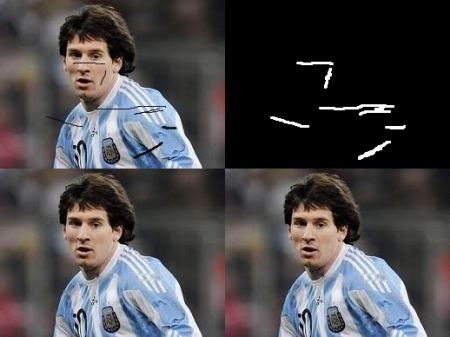
\includegraphics[width=0.8\textwidth]{inpainting-region.jpg}
\caption{Exemplo da seleção de regiões a serem preenchidas \cite{OpenCVmessi}. A imagem no canto superior esquerdo é a imagem danificada. No canto superior direito há a máscara (região) que selecionada pelo usuário para ser preenchida. A imagem no canto inferior esquerdo mostra a imagem após o processo de inpainting utilizando \cite{Bertalmio2001navier}, e a imagem no canto inferior direito mostra a imagem após o processo de inpainting utilizando \cite{Telea2004}.}
\label{fig:inpainting-region}
\end{figure}

\subsection{Inpainting inter-imagens} \label{inpainting-intra}

Os métodos clássicos possuem a vantagem de serem mais simples e rápidos, em especial, por utilizarem apenas as informações da própria imagem de entrada. Entretanto, ao se utilizar o aprendizado de máquina para completar imagens, é possível criar redes generativas, normalmente treinadas com um conjunto de dados maior, que podem gerar resultadas baseadas nas imagens que foram utilizadas para o treinamento.
\cite{li2017generative} e \cite{liao2018face} exploram este conceito na reconstrução de faces, um ``objeto'' que possui características únicas e que geralmente não pode ser gerado com outra região da imagem de entrada. Em sua técnica, \cite{li2017generative} o autor utiliza um modelo generativo, baseado em GANs, contendo um gerador e dois discriminadores. O gerador é responsável por completar as regiões faltantes da imagem, enquanto os discriminadores garantem que a área gerada é semanticamente coerente o realismo da imagem é mantido. A Figura \ref{fig:inpainting-inter} mostra um exemplo de inpainting inter-imagens.

\begin{figure}[ht]
\centering
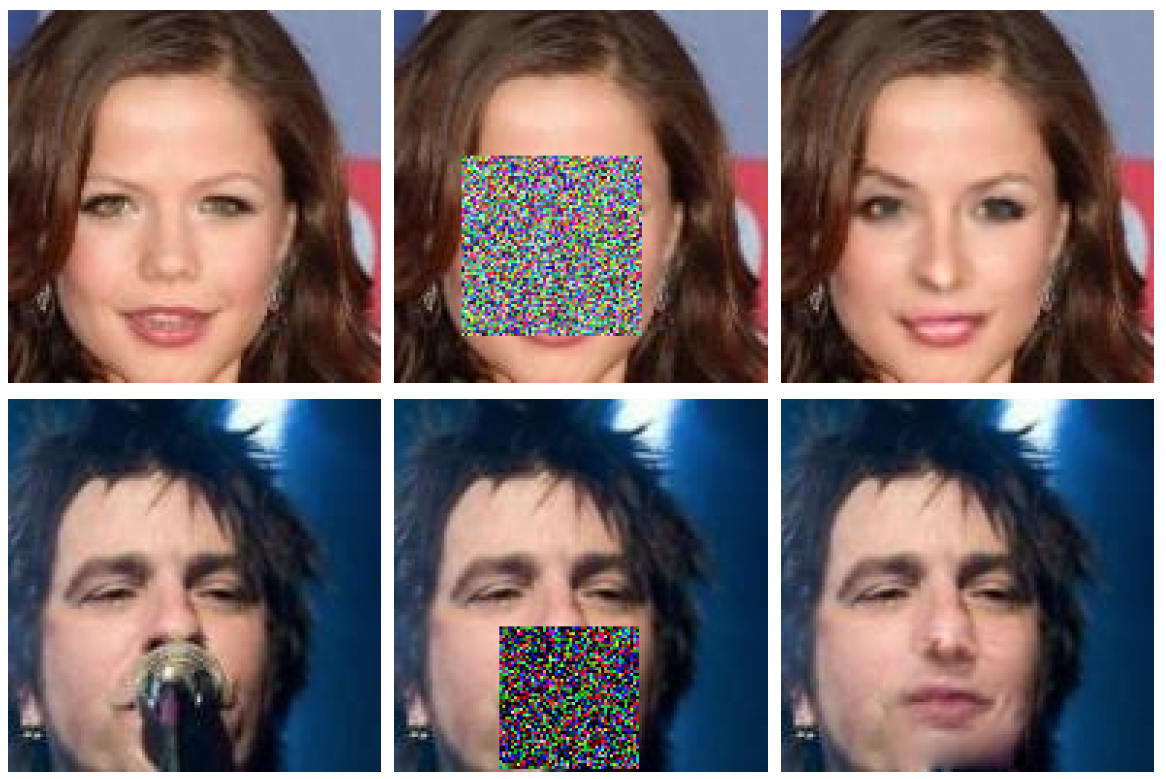
\includegraphics[width=0.8\textwidth]{inpainting-inter.jpg}
\caption{Adaptado de \cite{li2017generative}. As imagens à esquerda são a entrada. No centro, as máscaras da região a serem preenchidas são aplicadas. À direita estão resultados do processo de inpainting utilizando o método proposto pelo autor.}
\label{fig:inpainting-inter}
\end{figure}

Observa-se na Figura \ref{fig:inpainting-inter} que o método proposto pelo autor preenche as regiões com informações não presentes na imagem de entrada (mascarada), como por exemplo, a região dos olhos e da boca. 


\subsection{Depth Inpainting} \label{quality-depth}
O Depth Inpainting é uma técnica utilizada para realizar o inpainting de imagens 3D, como no caso de imagens obtidas por câmeras fotográficas ou sistemas de visão computacional. Esta técnica é útil em situações onde a câmera é incapaz de capturar corretamente as informações de profundidade, como é o caso de objetos translúcidos ou afetados pela luz especular (reflexos) \cite{shish20203dphoto}. 

De acordo com \cite{shish20203dphoto}, a técnica de Depth Inpainting consiste em utilizar uma rede neural convolucional para estimar a profundidade de uma imagem, treinada com imagens com values conhecidos, e então utilizar esta estimativa para completar a região faltante.
Outra abordagem é utilizar técnicas de processamento de imagens, como a interpolação de valores, para aproximar os values da região a ser preenchida. Isto pode ser obtido analisando os padrões e estruturas dos pixels vizinhos. Em ambos casos, o algoritmo precisa ser treinado com uma base de dados de imagens com valores de profundidade conhecidos para aprender a realizar predições.

% TODO: Algo sobre ML?

\section{Oportunidades de otimizações computacionais}

Em geral, o processo de complementar regiões faltantes é computacionalmente custoso, porque realiza-se grandes quantidades de cálculos para preencher as regiões selecionadas. Em especial, quando se é necessário processar várias imagens, imagens de alta resolução ou, ao depender da aplicação, o processo de inpainting pode necessitar ser realizado em tempo real, o que torna o tempo de processamento ainda mais importante. Por este motivo, é importante considerar as otimizações computacionais que podem ser realizadas para melhorar o desempenho da tarefa de preenchimento de imagens.

A programação paralela (do inglês, \emph{parallel processing}) é uma técnica de programação que permite a execução de múltiplos processos em paralelo, utilizando duas ou mais unidades de processamento \cite{tanenbaum2014os}. Para tal, é necessário que o algoritmo de inpainting seja capaz de dividir o processo em partes menores, que podem ser executadas em paralelo. Além disso, é necessário que o algoritmo seja capaz de combinar os resultados obtidos por cada parte do processo, para que o resultado final seja o mesmo que o obtido sem a utilização da programação paralela.
Normalmente, a programação paralela é utilizada para melhorar o desempenho de algoritmos que realizam cálculos intensivos e independentes entre si, como alguns algoritmos de processamento de imagens \cite{gonzalez2006image}.

O uso de placas gráficas, GPUs (do inglês, \emph{graphics processing units}), é uma estratégia que permite o uso das diversas unidades de processamento gráfico em uma GPU para realizar cálculos de processamento de imagens. As placas gráficas são unidades de processamento que possuem um grande número de núcleos de processamento (cores) e memória de alta velocidade, permitindo que elas sejam utilizadas para realizar cálculos de forma mais rápida que as CPUs, caso os cálculos necessários sejam simples, mas em volumosa quantidade. Além disso, as GPUs possuem um grande número de unidades de processamento, o que permite que o processamento seja realizado em paralelo, utilizando o conceito de programação paralela \cite{tanenbaum2014os}, mencionado anteriormente.

Existem diversas outras ténicas que podem ser utilizadas para melhorar o desempenho do processo de inpainting, como, por exemplo, a utilização de aproximações matemáticas, a redução da dimensão da imagem, o cálculo incremental, vetorização e instruções SIMD \cite{intel2022manual}, redução de redundância, otimização de acesso a memória e estruturas de dados. Por fim, implementá-las em uma linguagem de programação de alto desempenho, como C, C++ ou Rust, assim como o uso de ferramentas voltadas para aprendizado de máquina, como as linguagens R, Python, Julia, MATLAB e as bibliotecas PyTorch, Tensorflow \cite{tensorflow2015-whitepaper} e similares, pode ser uma boa estratégia para melhorar o desempenho do processo de inpainting.


\section{Trabalhos Relacionados} \label{related}

A Tabela \ref{related-works} apresenta, de forma resumida, os principais trabalhos relacionados ao tema deste trabalho, apresentando os seus objetivos, métodos e resultados.

% Referência | ano | Objetivo | Método | Resultado
% do not overflow the page width.
% break lines if necessary.
% use tabularx environment
\begin{table}[h]
\centering
\caption{Trabalhos relacionados ao tema deste trabalho.}
\label{related-works}
\begin{tabularx}{\linewidth}{|l|l|X|X|X|}
\hline
\textbf{Referência} & \textbf{Ano} & \textbf{Objetivo} & \textbf{Método} & \textbf{Resultado} \\
\hline
\cite{Bertalmio2000} & 2000 & Inpainting de imagens com texturas e estruturas simples. & Patch-based. & Imagens com texturas e estruturas simples. \\


\hline

\end{tabularx}
\end{table}








\section{Considerações Finais}\label{sec:conclusion}



Este relatório apresentou a aplicação dos métodos computacionais de diferenças finitas e de Runge-Kutta para a análise temporal do crescimento de uma ou mais populações em um sistema fechado. Esses métodos oferecem uma alternativa vantajosa em relação à solução analítica, que nem sempre é conhecida ou de fácil cálculo.

Para otimizar o desempenho dos algoritmos, foi necessário recorrer à biblioteca de compilação \emph{Just-In-Time} devido à quantidade de tempo necessária para computar os $N$ pontos de cada problema. Além disso, foi utilizada uma escolha particular para resolver a equação implícita do método de Euler Implícito, que aumentou drasticamente o tempo de execução do método. No entanto, se a equação implícita fosse resolvida antes da execução, o tempo gasto em um problema genérico se aproximaria do tempo do método de Euler Explícito. Como evidenciado pelos gráficos apresentados neste trabalho, o método de Euler Implícito é o que consome mais tempo para ser completamente executado.

Em resumo, a aplicação dos métodos computacionais estudados neste trabalho permite o início de uma resolução de problemas complexos do mundo real, oferecendo uma alternativa eficiente e acessível para aproximar numericamente soluções que nem sempre são conhecidas ou de fácil cálculo.
\section{Referências bibliográficas}
\begin{thebibliography}{99}
	
\bibitem{Bertalmio2000}
Bertalmio, M., Sapiro, G., Caselles, V., e Ballester, C. (2000). "Image inpainting". Proceedings of the 27th Annual Conference on Computer Graphics and Interactive Techniques — SIGGRAPH ’00.

\bibitem{Elharrouss2019}
Elharrouss, O., Almaadeed, N., Al-Maadeed, S., Akbari, Y. (2019). Image Inpainting: A Review. Neural Processing Letters.

\bibitem{Fontoura2022}
Fontoura, C. (2022). “Estudos De Métricas Para Quantificar Os Resultados De Aplicação De inpainting Para Melhoria Da Qualidade Do Processo De Extração De Feições Em Imagens Digitais”. Relatório de Qualificação de Doutorado, FCT-UNESP.

\bibitem{Dolhansky2018}
B. Dolhansky and C. C. Ferrer, "Eye In-painting with Exemplar Generative Adversarial Networks," 2018 IEEE/CVF Conference on Computer Vision and Pattern Recognition, 2018, pp. 7902-7911, doi: 10.1109/CVPR.2018.00824.

\bibitem{Bertalmio2001}
Bertalmio, M., Sapiro, G., Caselles, V.,  Ballester, C. (2001). Image inpainting. In Computer Graphics and Applications, 2001. Proceedings. 21st International Conference on (pp. 417-424). IEEE.

\bibitem{Criminisi2004}
Criminisi, A., Pérez, P., Toyama, K. (2004). Region filling and object removal by exemplar-based image inpainting. IEEE Transactions on image processing, 13(9), 1200-1212.

\bibitem{Efros1999}
Efros, A. A., Leung, T. K. (1999). Texture synthesis by non-parametric sampling. In Proceedings of the 26th annual conference on Computer graphicvs and interactive techniques (pp. 1033-1038). ACM.


\end{thebibliography}


\end{document}


